\documentclass{beamer}
\usepackage{tikz}
\usepackage{hyperref}
\usepackage{listings}
\usepackage{xcolor}

\lstset{
  basicstyle=\ttfamily\small,
  breaklines=true,
  columns=fullflexible,
  frame=single,
  backgroundcolor=\color{gray!10},
  keywordstyle=\color{blue},
  commentstyle=\color{green!50!black},
  stringstyle=\color{red!60!black},
  numberstyle=\tiny,
  numbers=left,
  numbersep=5pt,
  showspaces=false,
  showstringspaces=false,
  captionpos=b
}

\title{Campus Network Design and Implementation}
\subtitle{Computer Network-1 Course Project}
\author{Theodoros}
\institute{Contributors: }
\begin{document}

\begin{frame}
\titlepage
\end{frame}

\begin{frame}
\frametitle{Contents}
\begin{itemize}
    \item \hyperlink{design-diagram}{1. Network Design}
    \item \hyperlink{config}{2. Network Configuration}
    \item \hyperlink{routing}{3. Static/Dynamic Routing}
    \item \hyperlink{dhcp}{4. DHCP Configuration}
    \item \hyperlink{vlans}{5. VLAN Configuration}
    \item \hyperlink{testing}{6. Network Testing}
\end{itemize}
\end{frame}

\section{Network Design}
\begin{frame}[label=design-diagram]
\frametitle{Network Diagram}
\begin{center}
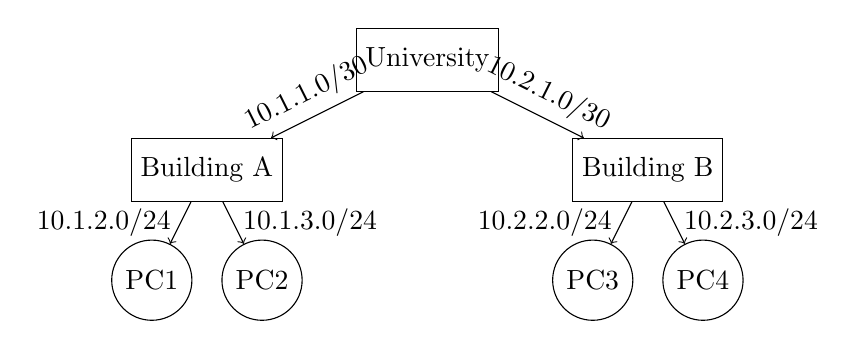
\begin{tikzpicture}[scale=0.7]
    \tikzstyle{router}=[draw, rectangle, minimum width=1.6cm, minimum height=0.8cm]
    \tikzstyle{pc}=[draw, circle, minimum width=0.9cm]
    \node[router] (r1) at (0,0) {University};
    \node[router] (r2) at (-4,-2) {Building A};
    \node[router] (r3) at (4,-2) {Building B};
    \draw[->] (r1) -- node[above,sloped]{10.1.1.0/30} (r2);
    \draw[->] (r1) -- node[above,sloped]{10.2.1.0/30} (r3);
    \node[pc] (pc1) at (-5,-4) {PC1};
    \node[pc] (pc2) at (-3,-4) {PC2};
    \draw[->] (r2) -- node[left]{10.1.2.0/24} (pc1);
    \draw[->] (r2) -- node[right]{10.1.3.0/24} (pc2);
    \node[pc] (pc3) at (3,-4) {PC3};
    \node[pc] (pc4) at (5,-4) {PC4};
    \draw[->] (r3) -- node[left]{10.2.2.0/24} (pc3);
    \draw[->] (r3) -- node[right]{10.2.3.0/24} (pc4);
\end{tikzpicture}
\end{center}
\end{frame}

\section{Network Configuration}
\begin{frame}[label=config]
\frametitle{Network Configuration}
\begin{itemize}
    \item MikroTik RouterOS is used for routers.
    \item Each router uses a unique identity and interface addressing.
    \item PCs have static IP addresses and default gateways.
    \item Subnetting: 10.1.x.x for Building A, 10.2.x.x for Building B.
\end{itemize}
\end{frame}

\begin{frame}[fragile]
\frametitle{Router Configuration: University Router (R1)}
\begin{lstlisting}
system identity set name="university"
ip address add address=10.1.1.1/30 interface=ether1
ip address add address=10.2.1.1/30 interface=ether2
\end{lstlisting}
\begin{itemize}
    \item Connects to Building A and B routers.
    \item /30 subnets for point-to-point links.
\end{itemize}
\end{frame}

\begin{frame}[fragile]
\frametitle{Router Configuration: Building A Router (R2)}
\begin{lstlisting}
system identity set name="Building_A"
ip address add address=10.1.1.2/30 interface=ether1
ip address add address=10.1.2.1/24 interface=ether2 
ip address add address=10.1.3.1/24 interface=ether3
\end{lstlisting}
\begin{itemize}
    \item ether1: Uplink to University Router
    \item ether2: First LAN subnet for PC1
    \item ether3: Second LAN subnet for PC2
\end{itemize}
\end{frame}

\begin{frame}[fragile]
\frametitle{Router Configuration: Building B Router (R3)}
\begin{lstlisting}
system identity set name="Building_B"
ip address add address=10.2.1.2/30 interface=ether1
ip address add address=10.2.2.1/24 interface=ether2    
ip address add address=10.2.3.1/24 interface=ether3
\end{lstlisting}
\begin{itemize}
    \item ether1: Uplink to University Router
    \item ether2: First LAN subnet for PC3
    \item ether3: Second LAN subnet for PC4
\end{itemize}
\end{frame}

\begin{frame}[fragile]
\frametitle{PC Configuration: Building A}
\begin{lstlisting}
# PC1
PC1> ip 10.1.2.2/24 10.1.2.1
# PC2
PC2> ip 10.1.3.2/24 10.1.3.1
\end{lstlisting}
\begin{itemize}
    \item Each PC has a static IP and gateway.
    \item Test: \texttt{ping 10.1.2.1} or \texttt{ping 10.1.3.1}
\end{itemize}
\end{frame}

\begin{frame}[fragile]
\frametitle{PC Configuration: Building B}
\begin{lstlisting}
# PC3
PC3> ip 10.2.2.2/24 10.2.2.1
# PC4
PC4> ip 10.2.3.2/24 10.2.3.1
\end{lstlisting}
\begin{itemize}
    \item Each PC has a static IP and gateway.
    \item Test: \texttt{ping 10.2.2.1} or \texttt{ping 10.2.3.1}
\end{itemize}
\end{frame}

\section{Static/Dynamic Routing}

\begin{frame}[fragile,label=routing]
\frametitle{RIP Configuration: University Router}
\begin{lstlisting}
# Enable RIP on relevant interfaces
routing rip interface add interface=ether1 send=v2 receive=v2
routing rip interface add interface=ether2 send=v2 receive=v2
# Tell RIP about directly connected subnets
routing rip network add network=10.1.1.0/30
routing rip network add network=10.2.1.0/30
# Set RIP settings
routing rip set redistribute-connected=yes
routing rip set update-timer=15s
routing rip set timeout-timer=30s
routing rip set garbage-timer=30s
\end{lstlisting}
\end{frame}

\begin{frame}[fragile]
\frametitle{RIP Configuration: Building A Router}
\begin{lstlisting}
routing rip interface add interface=ether1 send=v2 receive=v2
routing rip interface add interface=ether2 send=v2 receive=v2
routing rip interface add interface=ether3 send=v2 receive=v2
routing rip network add network=10.1.1.0/30
routing rip network add network=10.1.2.0/24
routing rip network add network=10.1.3.0/24
routing rip set redistribute-connected=yes
routing rip set update-timer=15s
routing rip set timeout-timer=30s
routing rip set garbage-timer=30s
\end{lstlisting}
\end{frame}

\begin{frame}[fragile]
\frametitle{RIP Configuration: Building B Router}
\begin{lstlisting}
routing rip interface add interface=ether1 send=v2 receive=v2
routing rip interface add interface=ether2 send=v2 receive=v2
routing rip interface add interface=ether3 send=v2 receive=v2
routing rip network add network=10.2.1.0/30
routing rip network add network=10.2.2.0/24
routing rip network add network=10.2.3.0/24
routing rip set redistribute-connected=yes
routing rip set update-timer=15s
routing rip set timeout-timer=30s
routing rip set garbage-timer=30s
\end{lstlisting}
\end{frame}

\begin{frame}[fragile]
\frametitle{RIP Command Explanations}
\begin{itemize}
    \item \texttt{routing rip interface add interface=etherX send=v2 receive=v2:} Enables RIP version 2 on the router’s interface. Only interfaces used to connect other routers should run RIP.
    \item \texttt{routing rip network add network=10.X.X.0/YY:} Informs RIP which directly-connected networks to advertise to neighbors.
    \item \texttt{routing rip set redistribute-connected=yes:} Ensures directly-connected networks are included in RIP updates.
    \item \texttt{routing rip set update-timer=15s:} How often RIP sends updates (default = 30s; lower for lab/small network).
    \item \texttt{routing rip set timeout-timer=30s:} If no update is received in 30s, the route is considered invalid.
    \item \texttt{routing rip set garbage-timer=30s:} A route is removed 30s after being marked invalid.
\end{itemize}
\end{frame}

\begin{frame}[fragile]
\frametitle{Verification: End-to-End Connectivity with RIP}
\textbf{Ping from PC3 to PC2 (Building B to Building A):}
\begin{lstlisting}
PC3> ping 10.1.3.2

84 bytes from 10.1.3.2 icmp_seq=1 ttl=61 time=1.491 ms
84 bytes from 10.1.3.2 icmp_seq=2 ttl=61 time=1.291 ms
84 bytes from 10.1.3.2 icmp_seq=3 ttl=61 time=2.439 ms
\end{lstlisting}
\textbf{Ping from PC1 to PC4 (Building A to Building B):}
\begin{lstlisting}
PC1> ping 10.2.3.2

84 bytes from 10.2.3.2 icmp_seq=1 ttl=61 time=1.831 ms
84 bytes from 10.2.3.2 icmp_seq=2 ttl=61 time=1.235 ms
84 bytes from 10.2.3.2 icmp_seq=3 ttl=61 time=2.860 ms
\end{lstlisting}
\textit{Successful replies indicate full network reachability via dynamic routing.}
\end{frame}

\section{DHCP Configuration}

\begin{frame}[fragile,label=dhcp-university]
\frametitle{DHCP: University Router}
\begin{lstlisting}
ip pool add name=pool1 ranges=10.1.1.2-10.1.1.2
ip pool add name=pool2 ranges=10.2.1.2-10.2.1.2

ip dhcp-server add interface=ether1 address-pool=pool1 \
  lease-time=24h name=dhcp1 disabled=no
ip dhcp-server add interface=ether2 address-pool=pool2 \
  lease-time=24h name=dhcp2 disabled=no

ip dhcp-server network add address=10.1.1.0/30 \
  dns-server=8.8.8.8,8.8.4.4 gateway=10.1.1.1
ip dhcp-server network add address=10.2.1.0/30 \
  dns-server=8.8.8.8,8.8.4.4 gateway=10.2.1.1

ip dhcp-server enable 0
ip dhcp-server enable 1
\end{lstlisting}
\end{frame}

\begin{frame}[fragile,label=dhcp-university-explanation1]
\frametitle{DHCP University Router: Command Explanations (1/2)}
\begin{itemize}
    \item \texttt{ip pool add ...} \\
    Creates a pool (range) of IP addresses that the DHCP server can assign to clients, excluding addresses statically set on routers.
    \item \texttt{ip dhcp-server add ...} \\
    Enables a DHCP server on a specific interface, using the defined pool. \texttt{lease-time=24h} means each client keeps its IP for 24 hours.
    \item \texttt{name=dhcpX} \\
    Used to identify different DHCP servers per interface (e.g., \texttt{dhcp1} for ether1, \texttt{dhcp2} for ether2).
\end{itemize}
\end{frame}

\begin{frame}[fragile,label=dhcp-university-explanation2]
\frametitle{DHCP University Router: Command Explanations (2/2)}
\begin{itemize}
    \item \texttt{ip dhcp-server network add ...} \\
    Specifies the subnet, default gateway, and DNS servers (here, Google DNS) to inform clients.
    \item \texttt{ip dhcp-server enable X} \\
    Activates the DHCP server instance (replace \texttt{X} with the correct number).
    \item \texttt{ip dhcp-server print} \\
    Shows the current DHCP servers configured on the router.
    \item \texttt{ip dhcp-server lease print} \\
    Displays the list of IPs assigned to clients.
\end{itemize}
\end{frame}

\begin{frame}[fragile,label=dhcp-building-a]
\frametitle{DHCP: Building A Router}
\begin{lstlisting}
ip address add address=10.1.2.1/24 interface=ether2
ip address add address=10.1.3.1/24 interface=ether3

ip pool add name=pool-buildingA1 ranges=10.1.2.100-10.1.2.200
ip pool add name=dhcp-pool-buildingA2 ranges=10.1.3.100-10.1.3.200

ip dhcp-server network add address=10.1.2.0/24 \
  gateway=10.1.2.1 dns-server=8.8.8.8
ip dhcp-server network add address=10.1.3.0/24 \
  gateway=10.1.3.1 dns-server=8.8.8.8

ip dhcp-server add interface=ether2 name=dhcp-buildingA1 \
  address-pool=pool-buildingA1
ip dhcp-server add interface=ether3 name=dhcp-buildingA2 \
  address-pool=dhcp-pool-buildingA2
ip dhcp-server enable dhcp-buildingA1
ip dhcp-server enable dhcp-buildingA2
\end{lstlisting}
\end{frame}

\begin{frame}[fragile,label=dhcp-building-b]
\frametitle{DHCP: Building B Router}
\begin{lstlisting}
ip address add address=10.2.2.1/24 interface=ether2
ip address add address=10.2.3.1/24 interface=ether3

ip pool add name=pool-buildingB1 ranges=10.2.2.100-10.2.2.200
ip pool add name=dhcp-pool-buildingB2 ranges=10.2.3.100-10.2.3.200

ip dhcp-server network add address=10.2.2.0/24 \
  gateway=10.2.2.1 dns-server=8.8.8.8
ip dhcp-server network add address=10.2.3.0/24 \
  gateway=10.2.3.1 dns-server=8.8.8.8

ip dhcp-server add interface=ether2 name=dhcp-buildingB1 \
  address-pool=pool-buildingB1
ip dhcp-server add interface=ether3 name=dhcp-buildingB2 \
  address-pool=dhcp-pool-buildingB2
ip dhcp-server enable dhcp-buildingB1
ip dhcp-server enable dhcp-buildingB2
\end{lstlisting}
\end{frame}

\begin{frame}[fragile,label=dhcp-test-pc]
\frametitle{DHCP Test: PC Example}
\begin{lstlisting}
# On PC in Building A, subnet 10.1.3.0/24:
PC2> ip dhcp
# Expected: IP 10.1.3.x/24, GW 10.1.3.1

# On PC in Building B, subnet 10.2.2.0/24:
PC3> ip dhcp
# Expected: IP 10.2.2.x/24, GW 10.2.2.1
\end{lstlisting}
\end{frame}

\section{VLAN Configuration}

\begin{frame}[fragile,label=vlans]
\frametitle{VLAN Configuration: Building A}
\begin{lstlisting}
interface vlan add name=vlan10 vlan-id=10 interface=ether2 disabled=no
interface vlan add name=vlan20 vlan-id=20 interface=ether3 disabled=no

ip address add address=10.1.2.1/24 interface=vlan10
ip address add address=10.1.3.1/24 interface=vlan20

ip address remove [find where interface=ether2]
ip address remove [find where interface=ether3]

interface vlan print
ip address print
\end{lstlisting}
\begin{itemize}
    \item vlan10 on ether2: Subnet 10.1.2.0/24 (e.g., PC1, webterm, PC7)
    \item vlan20 on ether3: Subnet 10.1.3.0/24 (e.g., PC6)
    \item Only VLAN interfaces have subnet IPs; physical interfaces do not.
\end{itemize}
\end{frame}

\begin{frame}[fragile]
\frametitle{Switch1 Configuration: Building A VLANs}
\begin{lstlisting}
Example Switch1 configuration (for VLAN 10/20)
 Port 0: dot1q trunk (to Router ether2/ether3)
 Port 1: VLAN 10 access (to PC1)
 Port 2: VLAN 10 access (to webterm)
 Port 3: VLAN 10 access (to PC7)

Port | VLAN | Type
0    | 1    | dot1q   # trunk to router ether2/ether3
1    | 10   | access  # PC1
2    | 10   | access  # webterm
3    | 10   | access  # PC7
\end{lstlisting}
\end{frame}

\begin{frame}[fragile,label=vlans-b]
\frametitle{VLAN Configuration: Building B}
\begin{lstlisting}
interface vlan add name=vlan30 vlan-id=30 interface=ether2 disabled=no
interface vlan add name=vlan40 vlan-id=40 interface=ether3 disabled=no

ip address add address=10.2.2.1/24 interface=vlan30
ip address add address=10.2.3.1/24 interface=vlan40

ip address remove [find where interface=ether2]
ip address remove [find where interface=ether3]

interface vlan print
ip address print
\end{lstlisting}
\begin{itemize}
    \item vlan30 on ether2: Subnet 10.2.2.0/24 (e.g., PC3)
    \item vlan40 on ether3: Subnet 10.2.3.0/24 (e.g., PC4, PC5)
    \item Only VLAN interfaces have subnet IPs; physical interfaces do not.
\end{itemize}
\end{frame}

\begin{frame}[fragile]
\frametitle{Switch2, Switch3, Switch4: Building B VLANs}
\begin{lstlisting}
# Switch2 configuration (Image 1)
Port | VLAN | Type
0    | 1    | dot1q
1    | 20   | access
2    | 20   | access
3-5  | 1    | access

# Switch3 configuration (Image 2)
Port | VLAN | Type
0    | 1    | dot1q
1    | 30   | access
2-5  | 1    | access

# Switch4 configuration (Image 3)
Port | VLAN | Type
0    | 1    | dot1q
1-2  | 40   | access
3-5  | 1    | access
\end{lstlisting}
\end{frame}

\begin{frame}[fragile]
  \frametitle{VLAN Configuration Testing \& Verification}
  \begin{itemize}
      \item \texttt{interface vlan print} \\
      Confirms VLAN interfaces and their status.
      \item \texttt{ip address print} \\
      Shows all IP assignments, ensuring only VLANs have subnet addresses.
      \item Connect PCs to correct VLAN and confirm DHCP works.
      \item \texttt{ping <gateway>} from a PC to verify connectivity.
  \end{itemize}
  \end{frame}
  
  \section{Network Testing}

  \begin{frame}[fragile,label=testing-dhcp]
  \frametitle{Network Testing: DHCP Assignment}
  \begin{lstlisting}
  PC7> ip dhcp
  DORA IP 10.1.2.99/24 GW 10.1.2.1
  PC6> ip dhcp
  DORA IP 10.1.3.200/24 GW 10.1.3.1
  PC3> ip dhcp
  DORA IP 10.2.2.200/24 GW 10.2.2.1
  PC5> ip dhcp
  DORA IP 10.2.3.200/24 GW 10.2.3.1
  PC4> ip dhcp
  DORA IP 10.2.3.199/24 GW 10.2.3.1
  \end{lstlisting}
  \begin{itemize}
      \item Each PC receives the correct IP address and gateway via DHCP.
  \end{itemize}
  \end{frame}
  
  \begin{frame}[fragile,label=testing-ping]
  \frametitle{Network Testing: Inter-VLAN/Inter-Building Connectivity}
  \begin{lstlisting}
  PC7> ping 10.1.2.1
  84 bytes from 10.1.2.1 icmp_seq=1 ttl=64 time=0.327 ms
  
  PC6> ping 10.1.2.99
  84 bytes from 10.1.2.99 icmp_seq=1 ttl=63 time=1.741 ms
  
  PC3> ping 10.1.2.99
  84 bytes from 10.1.2.99 icmp_seq=1 ttl=61 time=1.478 ms
  
  PC5> ping 10.1.3.200
  84 bytes from 10.1.3.200 icmp_seq=1 ttl=61 time=2.051 ms
  
  PC4> ping 10.1.2.99
  84 bytes from 10.1.2.99 icmp_seq=1 ttl=61 time=2.036 ms
  PC4> ping 10.1.2.3
  84 bytes from 10.1.2.3 icmp_seq=1 ttl=61 time=1.390 ms
  \end{lstlisting}
  \begin{itemize}
      \item All ping tests successful, showing inter-building and inter-VLAN routing with DHCP and VLANs.
  \end{itemize}
  \end{frame}

\end{document}